\section{Quantifying the impact of data center placement on power grid}
\label{sec:quantify}

Before studying the issues of data center placement in smart grid, it is crucial to look at and quantify the impact of different placement choices. In this section, we attempt to simulate the effects of putting data centers into the power grid with/without wind farms, and see how it will affect the grid in terms of transimission losses.

To quantify and compare the effects of different cases, we use following three metrics:

\begin{itemize}

\item \emph{Transimission Losses}.  When electricity is transmitted from generator to distribution network areas, some amount will be lost during the transimission. In general, losses can be estimated from the difference between produced power and the consumed power, assuming no theft of utility. Reducing the losses is important for the power grid to improve overall system efficiency and thereby reduce the cost of generated power.

\item \emph{Line capacity violation}. For a transimission line (referred as branch hereafter in the paper) in the grid system, the amount of power can be sent through it will be limited, depending on the length of the branch. A line has typically three ratings: short-term capacity rating, long-term capacity rating and rated capacity rating. If the power exceeds the minimum line capacity rating then one of the following will be done: i) the line is removed out of service; ii) the power flow is altered using some power electronic devices in the grid; or iii) generation and loads are interrupted. Thus, it's important to keep the line limit unviolated for the grid to work normally.

\item \emph{Voltage violation}. Voltage stability is very important for the performance of the grid system. Normally a voltage magnitude of 1.0 p.u. is considered to be favorable \cite{Seifi11}. For load buses, a range of 0.95-1.05 p.u. could be considered acceptable. If the bus voltage goes out of the range, we regard the system as voltage unstable. 
\xynote{This can hardly be observed, and didn't occur in the following experiments. But we are simulating a transimission network, right? how to demonstrate distribution network?}

\end{itemize}

\subsection{Setup}
To quantify the effect of placing datacentes into different locations of the power grid system, we study a situation where a transimission system has five wind farm installation and several large-scale data centers connected to the buses.

\subsubsection{Transimission network}
In our experiments, we are using a reduced order model of the existing New England transmission network, as shown in Figure~\ref{fig:newengland}.\xynote{should we re-draw this figure by ourselves??} This is a well-known bus system \cite{bills1970line} as which consists of 10 generators, 19 loads and 46 lines and transforms. The 10 generator buses are numbered from 30-39 in Figure~\ref{fig:newengland}, where bus 31 is a slack bus. Specifically, bus 39 represents the aggregation of a large number of generators interconnected to rest of US/Canada. 

%%%
\begin{figure}[ht]
\centering
\includegraphics[width=1\columnwidth]{img/newEngland.jpg}
\caption{New England 39 bus network}
\label{fig:newengland}
\end{figure}
%%%

During our simulation experiments, we compute the power flow for two kinds of system loads: \textsl{nominal} and \textsl{peak}, corresponding to the normal load  and the highest load throughout a whole year respectively. Note that the network constraints will become tight when facing peak load, where violations are more common to occur.

\subsubsection{Data center model}
Besides the grid system load, we also put the loads of data centers into the grid network, based on the geographical mapping according to \cite{DCmap}. We use six datacenters representing six states in New England, and the size setting of them is listed in Table~\ref{tab:dc_setting}. Note that here each data center represents the total load of data centers in the whole state. In order to estimate the size of an "aggregated" data center in a certain state, the follow equation is used:

\begin{equation}
L_i=\frac{n_i*9.8GW}{1278}
\end{equation}

\noindent where $L_i$ is the aggregated load of the $i$th state, $n_i$ is the number of datacenters reported in that state,  9.8GW is the upper bound of total electricity used by US data centers in 2010, according to the report \cite{Koomey2011}, and 1278 is the number of datacenters in US collected and reported in \cite{DCmap}. However, according to \cite{Koomey2011}, for the summarized load of data centers, there is an increase of 56\% from 2005-2010. Hence, we are assuming the increasing percentage from 2010-2014 is 56\%*0.8=45\%, and after adjustment we are using $L'_i=1.45L_i$ as the data center load for the target grid system. Besides, the data centers are mapped to different buses according to their geographical locations, which can also be found in Table~\ref{tab:dc_setting}.

\begin{table}[ht]
\begin{center}
\caption{Background data center load and location settings}
\begin{tabular}{|l|l|p{30pt}|p{30pt}|p{30pt}|}
\hline
DC No. & State & Number of DCs & Estimated size(MW) & Mapped Bus No.\\
\hline
DC1 & Connecticut & 12 &133.43 & 6\\
DC2 & Maine & 3 &33.36 & 29 \\
DC3 & Vermont & 4 &44.48 & 25 \\
DC4 & Rhode Island & 3 &33.36 & 20\\
DC5 & New Hampshire & 4& 44.48 & 16\\
DC6 & Massachusetts & 27& 300.21 & 4 \\
\hline

\end{tabular}
   \vspace{.05in}
\label{tab:dc_setting}
\end{center}
\end{table}


\subsubsection{Renewable energy}
To model renewable energy power installation, we use data collected from five wind farms located in New England area. \xynote{(Where is the data derived from?)} As Figure~\ref{fig:newengland} shows, they are connected to bus 18, 28, 36, 37 and 38 respectively. The locations and capacity settings of the 5 wind farms can be found in Table~\ref{tab:wf_setting}. As we know, the amount of wind power generation is mainly determined by the wind speed. For a GE 1.5MW wind turbine \cite{lei2006modeling}, the cut-in speed is between 4-5m/s, and the cut-off speed is 25m/s. The power generation approaches the rated capacity when the wind speed rises up to around 13m/s. The power curve of a GE 1.5MW turbine we used in this study is as shown in Fig.\ref{fig:windcurve}. In the follow experiments, we classify the wind speeds into four categories: ZERO (0-3m/s), LOW (4-6m/s), MEDIUM (7-11m/s), and HIGH ($>$11m/s). \xynote{Why did we choose GE turbines? What's the assumption about aggregating turbines? I have no idea about these two questions. Do you have some suggestions?}

%%%
\begin{figure}[ht]
\centering
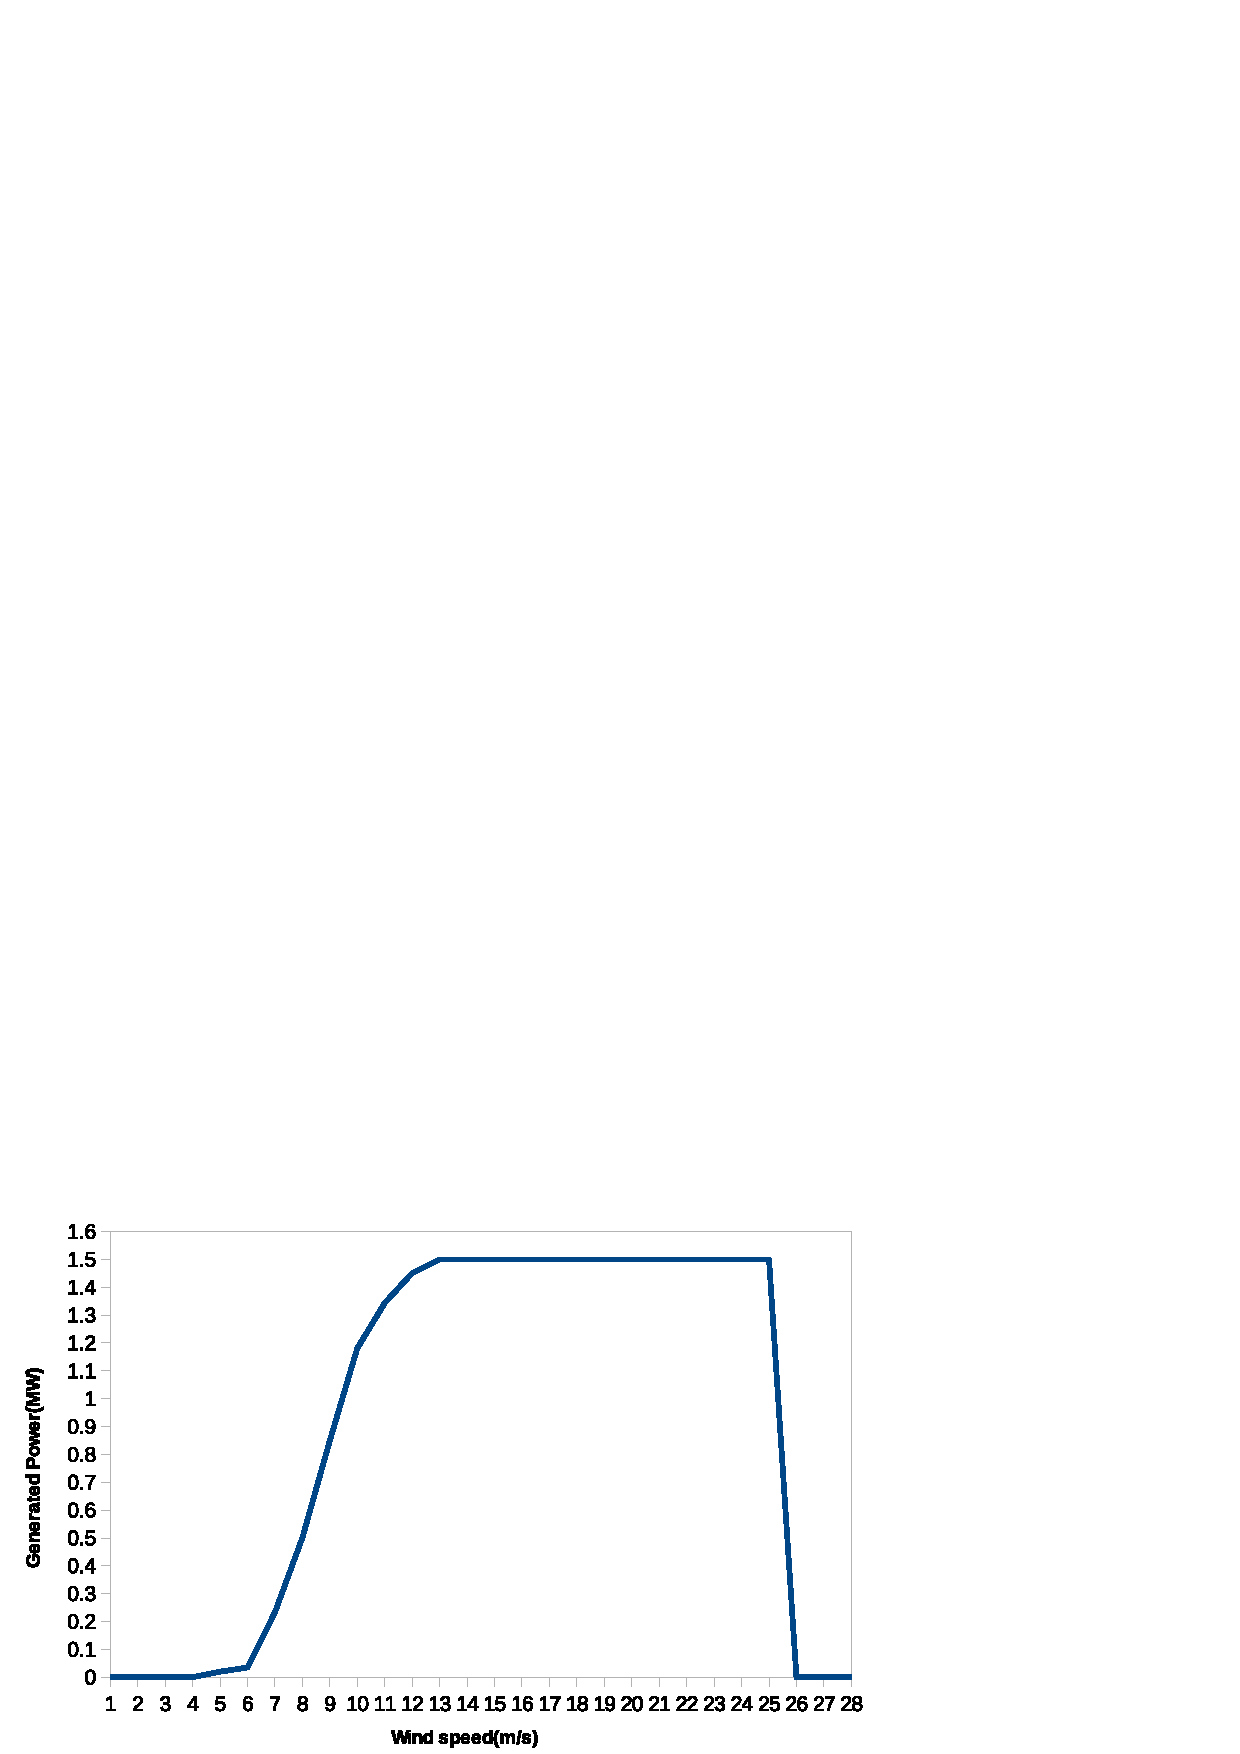
\includegraphics[width=1\columnwidth]{img/wind_curve.pdf}
\caption{Power curve of the GE 1.5MW wind turbine}
\label{fig:windcurve}
\end{figure}
%%%


\begin{table}[ht]
\begin{center}
\caption{Wind farm settings}
\begin{tabular}{|l|l|c|c|}
\hline
WF No. & Bus No. & State & Capacity(MW) \\
\hline
WF1 & 18& ? & 100\\
WF2 & 28& ? & 90 \\
WF3 & 36& Vermont & 90  \\
WF4 & 37& Maine & 90\\
WF5 & 30& Massachusetts(?) & 90\\
\hline

\end{tabular}
   \vspace{.05in}
\label{tab:wf_setting}
\end{center}
\end{table}


\subsection{Case study}
Based on the settings described above, we conduct simulation experiments to study the impact of data center placement at different locations on the performance and efficiency of the tested grid network. Furthermore, we also investigate the potential impact of data center capacity on the grid, and try to examine the effect of jointly placing a large-scale data center and a wind farm.

\subsubsection{Impact of data center location}
First, we attempt to conduct the study of the impact of connecting a new data center to different buses. Based on the basic configuration of the grid system with nominal load, including the existing 6 data centers and 5 wind farms, we try to establish a new  data center with the size of 100MW and put it into the grid network. Note that since we are doing a bulk transimission system study, this capacity could be the aggregated capacity of multiple data centers. Figure~\ref{fig:loc-loss} shows the comparison of total system losses when the extra data center locate on each bus from 1-39, under the condition of four different wind speed settings. 

%%%
%\begin{figure}[ht]
%\centering
%\includegraphics[width=0.8\columnwidth]{img/location-loss}
%\caption{Impact of data center locations on losses}
%\label{fig:loc-loss}
%\end{figure}
%%%

\begin{figure} [ht]
%\begin{tabular}{cc} 
\begin{subfigure}[b]{.22\textwidth}
%  \centering
  \includegraphics[width=4.5cm]{img/loc-loss-zero}
  \caption{ZERO}
  \label{fig:a:l-l-zero}
\end{subfigure}
\hfill
\begin{subfigure}[b]{.22\textwidth}
%  \centering
  \includegraphics[width=4.5cm]{img/loc-loss-low-new}
  \caption{LOW}
   \label{fig:b:l-l-low}
\end{subfigure}
%\vskip\baselineskip
\begin{subfigure}[b]{.22\textwidth}
 % \centering
  \includegraphics[width=4.5cm]{img/loc-loss-mid-new}
  \caption{MEDIUM}
   \label{fig:c:l-l-mid}
\end{subfigure}
\hfill
\begin{subfigure}[b]{.22\textwidth}
 % \centering
  \includegraphics[width=4.5cm]{img/loc-loss-high-new}
  \caption{HIGH}
   \label{fig:d:l-l-high}
\end{subfigure}
\caption{Impact of data center locations on losses}
\label{fig:loc-loss}
\end{figure}


As shown, the total system losses vary a lot when putting a new datacenter in different places. For example, when the wind speed setting is MEDIUM, the maximum loss (at bus 39) could be 14\% larger than the minimum value (at bus 38), and the standard deviation is 1.45. \xynote{we have changed the wind farm at bus 38 to bus 30, and updated the results in Fig.3. The results are similar as before. Is this OK to be used as a counter-productive example for co-location?} This highlights that choosing the place for a large-scale data center does greatly affect the power grid and provide the potential for helping the grid manager to save energy losses. 

Note that in the previous experiment there are no violations occuring, since the system load is far below the constraints. Next, we change the scenario to peak system load and conduct the simulation again in order to investigate the impact of data center placement on line capacity violations. Evaluation results are illustrated in Figure~\ref{fig:loc-vio}, which highlights that the number of violated branches is quite different when the data center is connected to different buses. In particular, take Figure~\ref{fig:c:l-v-mid} for example, there is only one branch violated when the data center is connected to bus 31, but 4 branches violated when it's connected to bus 14. 


\begin{figure} [ht]
%\begin{tabular}{cc} 
\begin{subfigure}[b]{.22\textwidth}
%  \centering
  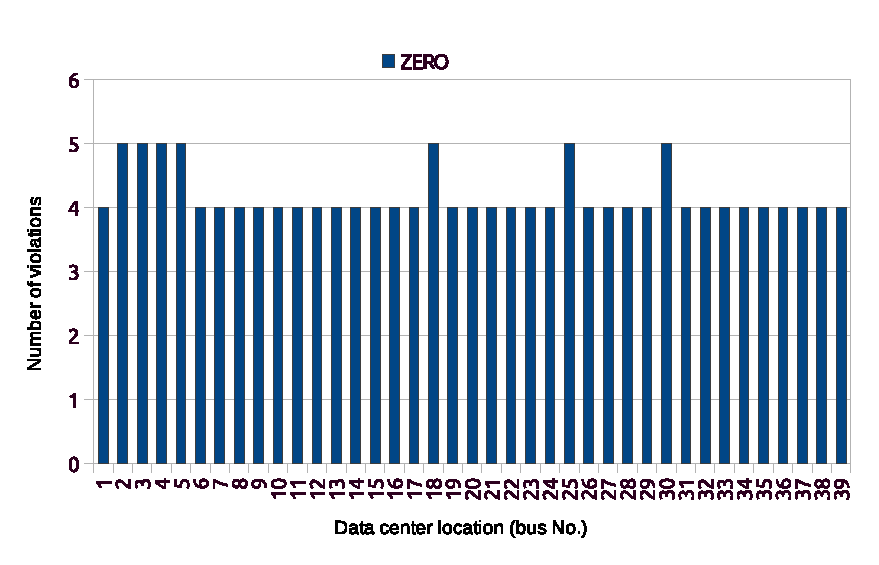
\includegraphics[width=4.3cm]{img/loc-vio-zero}
  \caption{ZERO}
  \label{fig:a:l-v-zero}
\end{subfigure}
\hfill
\begin{subfigure}[b]{.22\textwidth}
%  \centering
  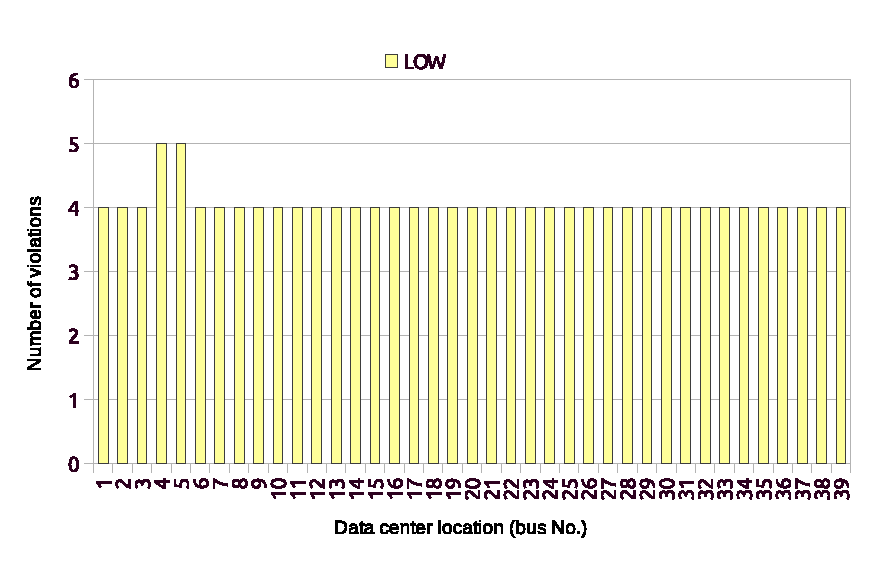
\includegraphics[width=4.3cm]{img/loc-vio-low}
  \caption{LOW}
   \label{fig:b:l-v-low}
\end{subfigure}
%\vskip\baselineskip
\begin{subfigure}[b]{.22\textwidth}
 % \centering
  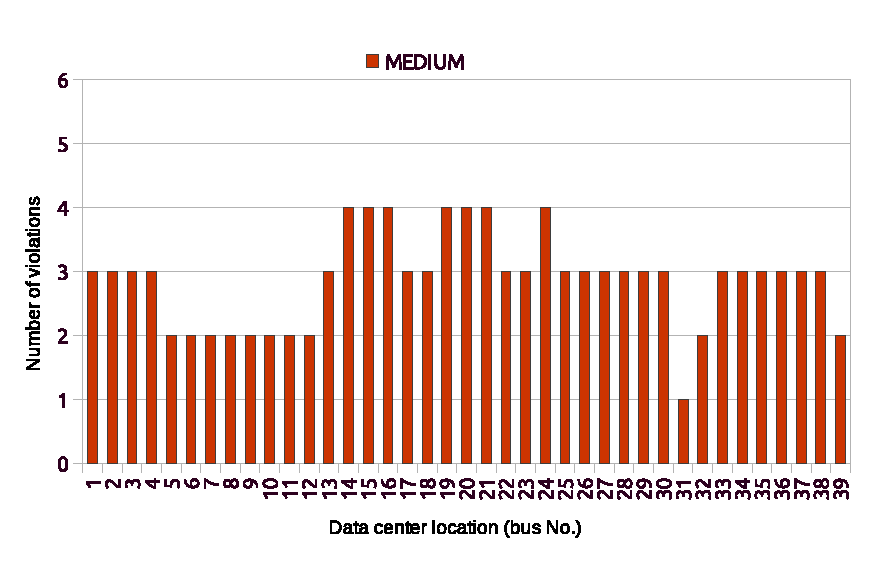
\includegraphics[width=4.3cm]{img/loc-vio-mid}
  \caption{MEDIUM}
   \label{fig:c:l-v-mid}
\end{subfigure}
\hfill
\begin{subfigure}[b]{.22\textwidth}
 % \centering
  \includegraphics[width=4.3cm]{img/loc-vio-high}
  \caption{HIGH}
   \label{fig:d:l-v-high}
\end{subfigure}
\caption{Impact of data center locations on violations}
\label{fig:loc-vio}
\end{figure}


\subsubsection{Impact of data center size}
Here, we set the wind speed of the five wind farms all to ZERO, LOW, MEDIUM and HIGH repectively and see how the data center size will affect the total power losses of the grid system. The added data center will be fixed on a certain bus location, and only the load of the data center varies. Figure~\ref{fig:dc_size_loss} shows the results under four scenarios corresponding to different wind speeds, when the data center is located at bus 1, 2, 18, 25, 31, 36, 38 and 39 respectively. Note that the eight buses were chosen out of 39 buses since they are representive for all kinds of variation types. 

\begin{figure*}[ht]
%\begin{tabular}{cc}   
\begin{minipage}{0.2\linewidth}
  \centerline{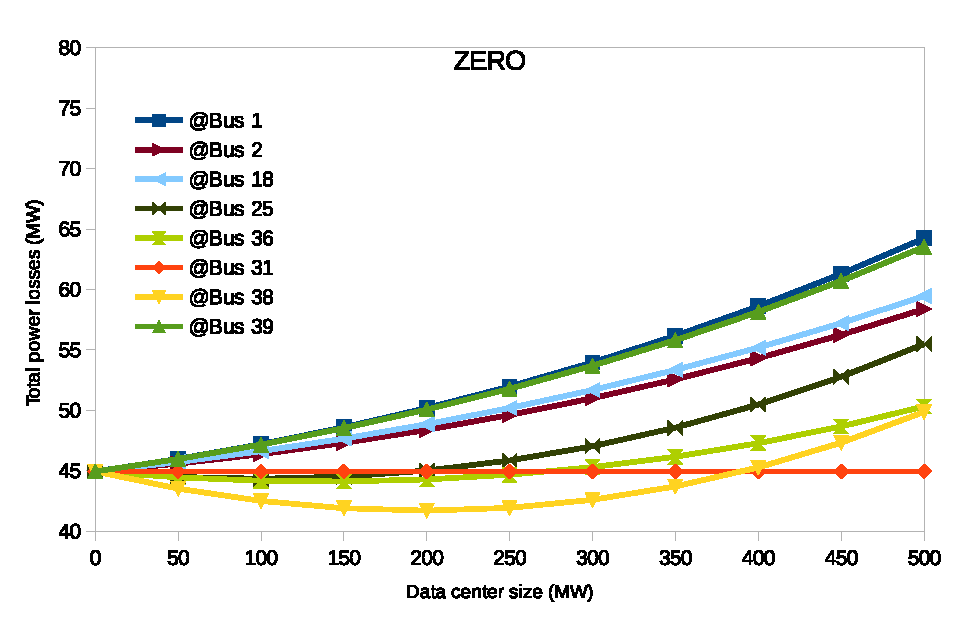
\includegraphics[width=5.0cm]{img/size-loss-zero}}
  \centerline{(a) Wind speed set to ZERO}
  \label{fig:a:zero}
\end{minipage}
\hfill
\begin{minipage}{.2\linewidth}
  \centerline{\includegraphics[width=5.0cm]{img/size-loss-low}}
  \centerline{(b) Wind speed set to LOW}
   \label{fig:b:low}
\end{minipage}
%\vfill
\hfill
\begin{minipage}{0.2\linewidth}
  \centerline{\includegraphics[width=5.0cm]{img/size-loss-mid}}
  \centerline{(c) Wind speed set to MEDIUM}
  \label{fig:c:medium}
\end{minipage}
\hfill
\begin{minipage}{0.2\linewidth}
  \centerline{\includegraphics[width=5.0cm]{img/size-loss-high}}
  \centerline{(d) Wind speed set to HIGH}
  \label{fig:d:high}
\end{minipage}
%\end{tabular}
\caption{Impact of data center sizes on losses.}
\label{fig:dc_size_loss}
\end{figure*}

From Figure~\ref{fig:dc_size_loss}a, we can see that the change of the data center load will affect the system performance obviously, with the total power losses varying from 44.9 MW to 64.2 MW. A more important finding is that, with the presence of wind farms, increasing the data center load would have different impact on the system losses when placed at different locations. For example, in Figure~\ref{fig:dc_size_loss}b and Figure~\ref{fig:dc_size_loss}c, it can be observed that, the losses increase as the load of the data center become heavier when the data center is placed at bus 1, 2, 18 and 39. However, when the data center is connected to bus 25, 36 or 38, there is a certain size for the data center to make the system losses achieving a minimal value. Since the load of the data center could be adjusted by a variety of techniques \cite{}, this implicates the possibility that it could be leveraged to confront the variability of the wind power generation, which could have negative effect to the grid network. It's also notable that no matter how large is the data center size, the losses keep constant if the data center is connected to bus 31. This is because bus 31 is a slack bus, which is used to balance the active and reactive power in the grid system by taking up any power mismatch between load and generation.

Furthremore, we also investigated the impact on the grid branches by changing the size of the data center. Figure~\ref{fig:dc_size_vio} shows the results when the data center with varying sizes is connected to bus 25 and 36 repectively. Results of other bus locations show similar characteristics and thus will be omitted here. It seems that the possibility of getting branches violated will become larger when the data center's load goes higher. On the other hand, it's notable that high wind speeds lead to fewer violations, which implicates that with wind power generation, the grid can tolerant higher load from data centers.


\begin{figure} [ht]
%\begin{tabular}{cc} 

\begin{subfigure}{0.23\textwidth}
  \centering
  \includegraphics[width=4.5cm]{img/size_vio_bus25}
  \caption{Data center at bus 25}
  \label{fig:a:bus25}
\end{subfigure}
%\hfill
\begin{subfigure}{.23\textwidth}
  \centering
  \includegraphics[width=4.5cm]{img/size_vio_bus36}
  \caption{Data center at bus 36}
   \label{fig:b:bus36}
\end{subfigure}
\caption{Impact of data center sizes on line capacity violations}
\label{fig:dc_size_vio}

\end{figure}

\subsubsection{Comparison before and after placing the data center and wind farm}

In order to investigate the impact of placing data center and wind farm into the grid network, we compare the losses of eight different cases, including BASE (the base grid network), DC (base grid with one 100MW data center), LOW\_WF, MED\_WF, HIGH\_WF (base grid with one extra wind farm set to LOW, MEDIUM, HIGH wind speed respectively), DC\&LOW\_WF, DC\&MED\_WF, DC\&HIGH\_WF (based grid with both data center and wind farm corresponding to different wind speed settings). The comparison results are illustrated in Figure~\ref{fig:add-on-cases}. It implies that  placing a data center at a proper location might help the grid with/without wind farms to reduce total power losses.


%%%
\begin{figure}[ht]
\centering
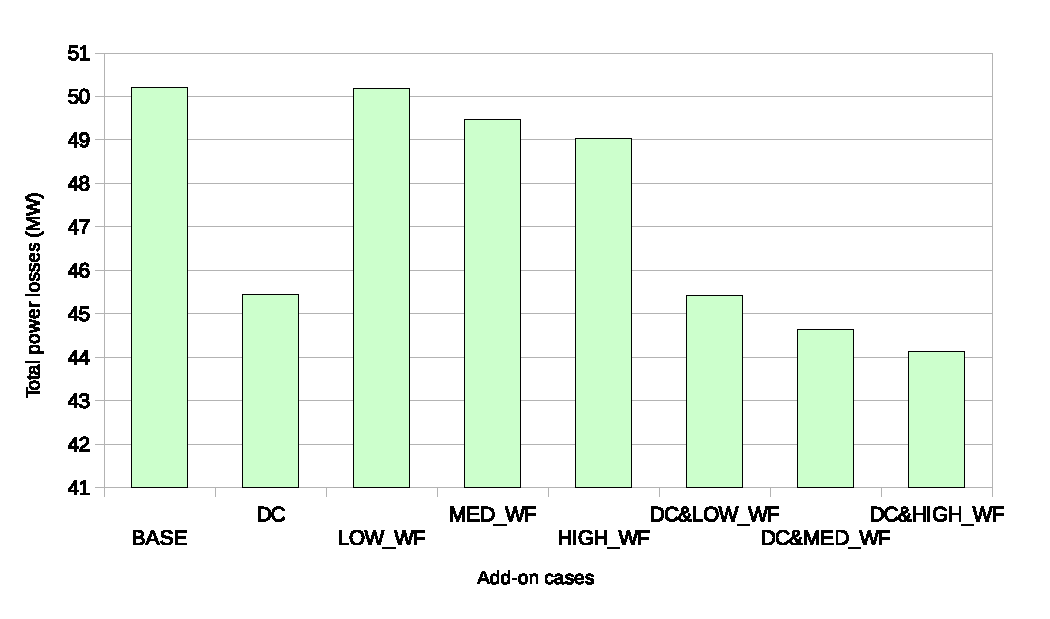
\includegraphics[width=.8\columnwidth]{img/add-on-cases}
\caption{Losses before and after data center and wind farm placement}
\label{fig:add-on-cases}
\end{figure}
%%%

\subsubsection{Jointly considering the placement of data center and wind farm}
Assuming that a new data center and a new wind farm will be established and connected into the power grid system, where is the best place for them to be constructed in order to bring least negative impact to the grid network? We try to examine the different effect of the following four stategies:

(1) \emph{Only DC}: We only consider the placement of the data center to minimize the power losses of the whole system, without the knowledge of wind farms.

(2) \emph{Only WF}: We only consider the placement of the wind farm to minimize the impact, without knowing about the data center.

(3) \emph{Co-location}: We put the data center and the wind farm together and connect both of them to the same bus.

(4) \emph{Jointly}: We jointly consider their impact together by comparing the situation when they are connected to different buses and try to find the best one of the combinations.

When the wind speed and the size of the data center are set to different values, the minimal losses could be different. We use the four strategy to find the place with minimum losses of the whole system, and the results are illustrated as in Figure~\ref{fig:joint_loss}. A main observation is that co-location is not a best choice in terms of reducing total power losses of the entire grid. Minimum losses are usually achieved when the data center and the wind farm are placed into different places.


%%%
\begin{figure}[ht]
\centering
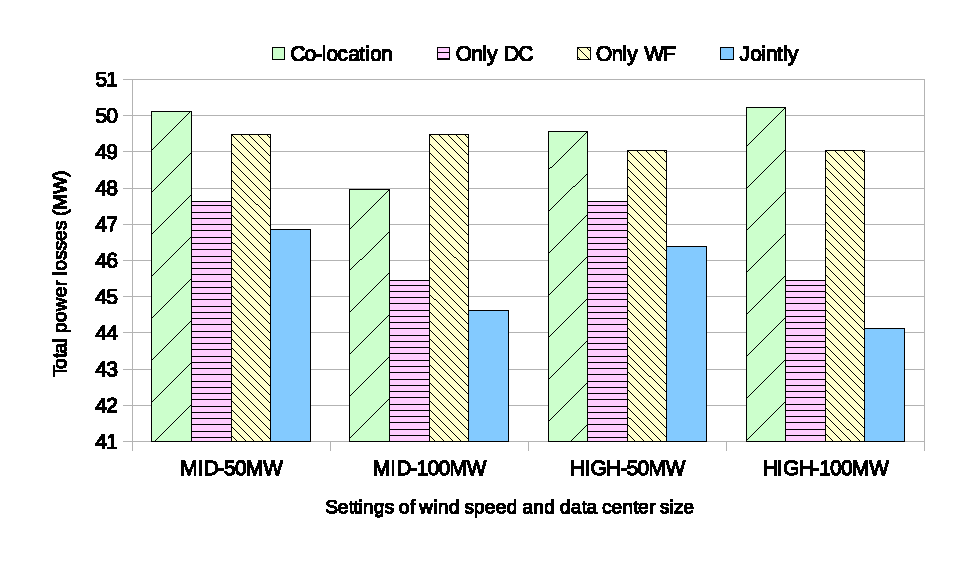
\includegraphics[width=1\columnwidth]{img/joint_loss}
\caption{Comparison of different placement choices}
\label{fig:joint_loss}
\end{figure}
%%%



%%%
%\begin{figure}[tb]
%\centering
%\includegraphics[width=1\columnwidth]{img/min_max_loss}
%\caption{Minumum and maximum transimission losses with different data center sizes}
%\label{fig:min_max_loss}
%\end{figure}
%%%
